\documentclass{article} 
\usepackage{url, graphicx}
\usepackage[margin=1in]{geometry}

\title{My Fantastic Article}
\author{Toni Farley}
\date{}

\begin{document}

\maketitle

\section{Introduction}

In this study, we queried dozens of individuals, and learned that none of them were familiar with \LaTeX!  We talked to many different kinds of people:

\begin{itemize}
\item Students
\item Researchers
\item Grandparents
\end{itemize}

\noindent When asked if they knew how to use \LaTeX, these are the responses we got:

\begin{enumerate}
\item What?
\item Who?
\item No
\end{enumerate}

In light of this shocking discovery, we decided to create this course. Fortunately, we were able to find an excellent resource for hosting our course online: \url{www.udemy.com}. We like udemy, and hope our students agree. So, we got busy on the most challenging part of this course development effort, and created a course graphic as shown in Figure~\ref{fig:course}.

\begin{figure}[htbp]
\begin{center}
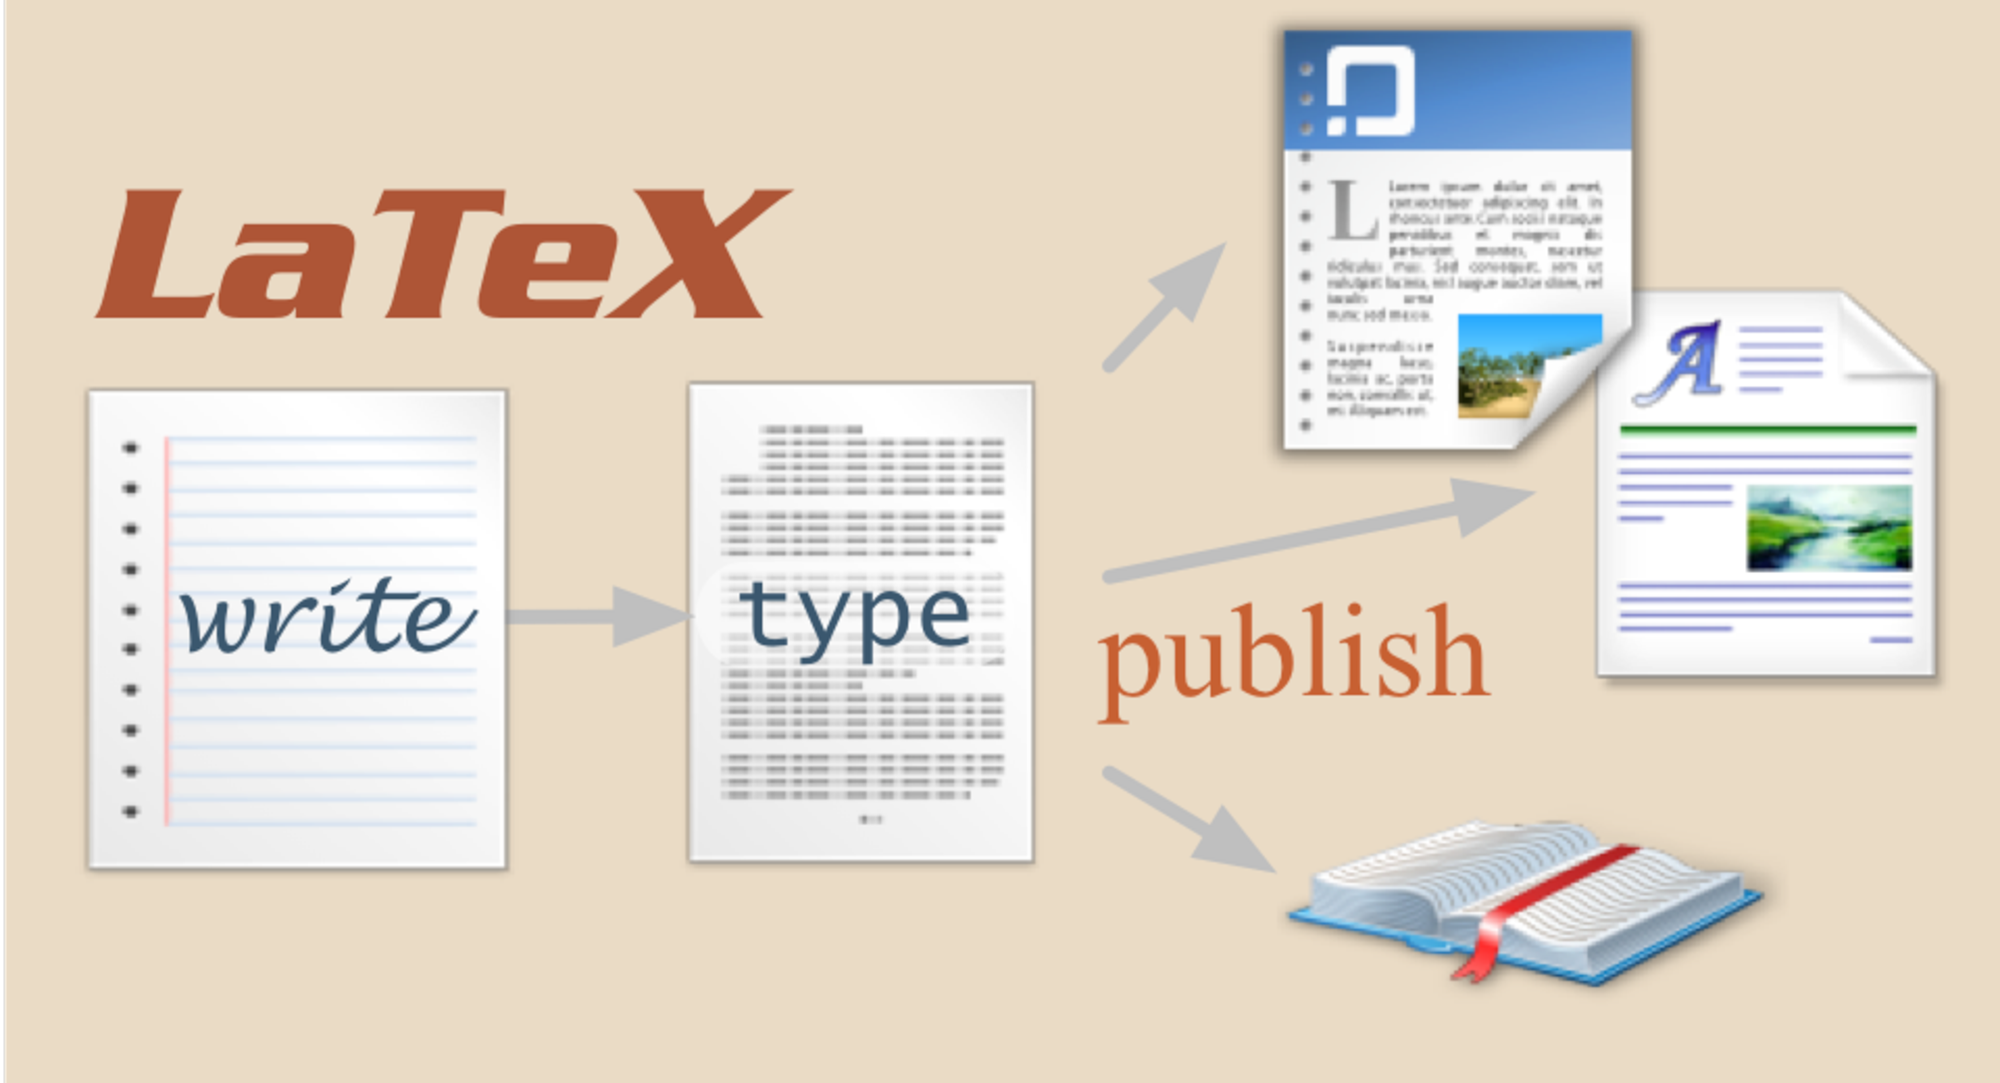
\includegraphics[width=3in]{course_graphic}
\caption{Our awesome course graphic.}
\label{fig:course}
\end{center}
\end{figure}

\section{Course}

There are many aspects to learning \LaTeX. Some are more challenging to learn than others. 

\subsection{Philosophy}

This course is introductory, and intended to get you started with the basics, but touch on some advanced topics as well. We focus on guiding you to resources online so you can continue learning beyond the content of this course.

\subsection{Content}

We organized our course into several content sections as shown in Table~\ref{tab:content}.

\begin{table}[h!]
\caption{Our course content.}
\begin{center}
\begin{tabular}{|c|c|}
\hline
Section & Title \\
\hline
1 & Getting Started\\
2 & Creating a New Document (.tex) \\
3 & Graphics and Tables \\
4 & Bibliography (.bib and .bbl) \\
5 & Elements in Science and Mathematics \\
6 & Managing Packages and Style Files (.sty) \\
7 & Advanced Topics \\
8 & Next Steps \\
\hline
\end{tabular}
\end{center}
\label{tab:content}
\end{table}%

\section{Conclusion}

This was a fun course to develop, and we hope you enjoy it!

\end{document} 